\begin{ccRefFunction}{compare_x_at_y}

\ccFunction{Comparison_result compare_x_at_y(const Point_2<Kernel> &p,
                                             const Line_2<Kernel> &h);}
        {compares the $x$-coordinates of $p$ and the horizontal projection
         of \ccStyle{p} on \ccStyle{h}%
         \ccTexHtml{ (Figure~\ref{fig-compare_x_at_y} (a))}{; see (a) in the 
         figure below}.
         \ccPrecond \ccStyle{h} is not horizontal.}

\begin{ccTexOnly}
\begin{figure}[h]
\centerline{
  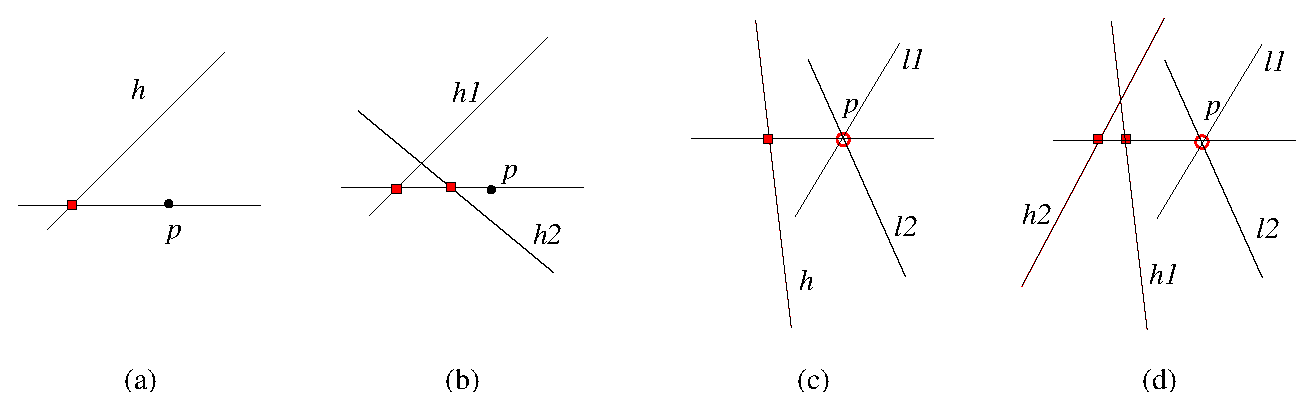
\includegraphics[width=\textwidth]{Kernel_23_ref/fig/compare_x_at_y}}
\caption{Comparison of the $x$-coordinates of the (implicitly given)
         points in the boxes, at a $y$-coordinate. The $y$-coordinate
         is either given explicitly (disc) or implicitly (circle).
         \label{fig-compare_x_at_y}}
\end{figure} 
\end{ccTexOnly} 

\ccFunction{Comparison_result compare_x_at_y(const Point_2<Kernel> &p,
                                             const Line_2<Kernel> &h1,
                                             const Line_2<Kernel> &h2);}
{This function compares the $x$-coordinates of the horizontal projection 
 of \ccStyle{p} on \ccStyle{h1} and on \ccStyle{h2}%
 \ccTexHtml{ (Figure~\ref{fig-compare_x_at_y} (b))}{; see (b) in the figure 
 below}.
\ccPrecond \ccStyle{h1} and \ccStyle{h2} are not horizontal.
}

\ccFunction{Comparison_result compare_x_at_y(const Line_2<Kernel> &l1,
                                           const Line_2<Kernel> &l2,
                                           const Line_2<Kernel> &h);}
      {Let $p$ be the \ccHtmlNoLinksFrom{intersection} of lines $l1$ and $l2$.
       This function compares the $x$-coordinates of $p$ and 
       the horizontal projection of \ccStyle{p} on \ccStyle{h}%
       \ccTexHtml{ (Figure~\ref{fig-compare_x_at_y} (c))}{; see (c) in the 
       figure below}.
       \ccPrecond \ccStyle{l1} and \ccStyle{l2} intersect and are not 
       horizontal; \ccStyle{h} is not horizontal.
}


\ccFunction{Comparison_result compare_x_at_y(const Line_2<Kernel> &l1,
                                             const Line_2<Kernel> &l2,
                                             const Line_2<Kernel> &h1,
                                             const Line_2<Kernel> &h2);}
{Let $p$ be the \ccHtmlNoLinksFrom{intersection} of lines $l1$ and $l2$. This 
 function compares the $x$-coordinates of the horizontal projection of 
 \ccStyle{p} on \ccStyle{h1} and on \ccStyle{h2}%
 \ccTexHtml{ (Figure~\ref{fig-compare_x_at_y} (d))}{; see (d) in the figure 
 below}.
\ccPrecond \ccStyle{l1} and \ccStyle{l2} intersect and are not horizontal; 
 \ccStyle{h1} and \ccStyle{h2} are not horizontal.
}

\begin{ccHtmlOnly}
<img border=0 src="fig/compare_x_at_y.gif" align=middle alt="Comparison of x at y"> 
\end{ccHtmlOnly} 

\ccSeeAlso
\ccRefIdfierPage{CGAL::compare_xy} \\
\ccRefIdfierPage{CGAL::compare_xyz} \\
\ccRefIdfierPage{CGAL::compare_x} \\
\ccRefIdfierPage{CGAL::compare_y} \\
\ccRefIdfierPage{CGAL::compare_yx} \\
\ccRefIdfierPage{CGAL::compare_y_at_x} \\
\ccRefIdfierPage{CGAL::compare_z} \\

\end{ccRefFunction}

